\documentclass[letterpaper,10pt,conference]{IEEEtran}
\usepackage[T1]{fontenc}
\usepackage{amsmath,amssymb,graphicx,booktabs,cite,url,xcolor,array}
\usepackage[hidelinks]{hyperref}
\newcommand{\R}{\mathbb{R}}
\newcommand{\crossmat}[1]{[#1]_{\times}}
\title{Adapting to Contact: Tactile Configuration of Virtual Mechanics}
\author{\IEEEauthorblockN{Anonymous authors}}
\begin{document}
\maketitle
\begin{abstract}
Contact location and object motion can be uncertain during occluded manipulation. We connect an eight-electrode electrical impedance tomography (EIT) interface to virtual model control (VMC): contact events select interaction phases, while contact location configures virtual attachments and corrects task progress. Synthetic UR3e simulations distinguish these effects. EIT attachment completes 27/27 joystick trials versus 9/27 for centre attachment, with mean peak contact force of 4.19 versus 5.61 N. During ball rolling, EIT position feedback reduces final position error after a push from 2.73 to 0.41 mm. Updating the attachment reduces maximum palm tilt from 4.01 to 1.92 degrees relative to initial-contact attachment at low orientation stiffness. Progress-bias tests connect sensing error to task tolerance. These results support task-specific benefits of EIT information within the implemented controllers; they do not establish general VMC superiority. Physical curved-contact calibration and hardware validation remain required.
\end{abstract}
\begin{IEEEkeywords}
Soft tactile sensing, electrical impedance tomography, virtual model control, contact adaptation.
\end{IEEEkeywords}

\section{Introduction}
A robot palm can hide its contact with a joystick or ball. Initial placement errors shift the contact away from the palm centre; rolling moves it across the pad, and slip changes the relationship between palm travel and ball motion. Contact detection alone cannot resolve these geometric and motion errors. Human fingertip experiments likewise show that somatosensory feedback adjusts force coordination to changed contact geometry~\cite{jenmalm}.

Virtual model control (VMC) represents interaction through virtual mechanical components and maps their forces to joint commands~\cite{pratt}. A tactile interface can determine when these components engage, where they attach, and how their internal task state is corrected (Fig.~\ref{fig:framework}). We examine those roles using EIT contact state and location, without feedback from its force estimate.

The contribution is an implemented EIT-to-VMC interface and matched simulation comparisons linking tactile information to task performance. Joystick operation tests defining the VMC attachment at contact. Ball rolling separates position correction after a disturbance from attachment updates during contact migration, and tests recovery after contact loss. Sensing perturbations identify limits of the tested controller. Object geometry is supplied; the contribution concerns uncertain contact on the palm. All reported task results are synthetic simulations.

\begin{figure*}[t]
\centering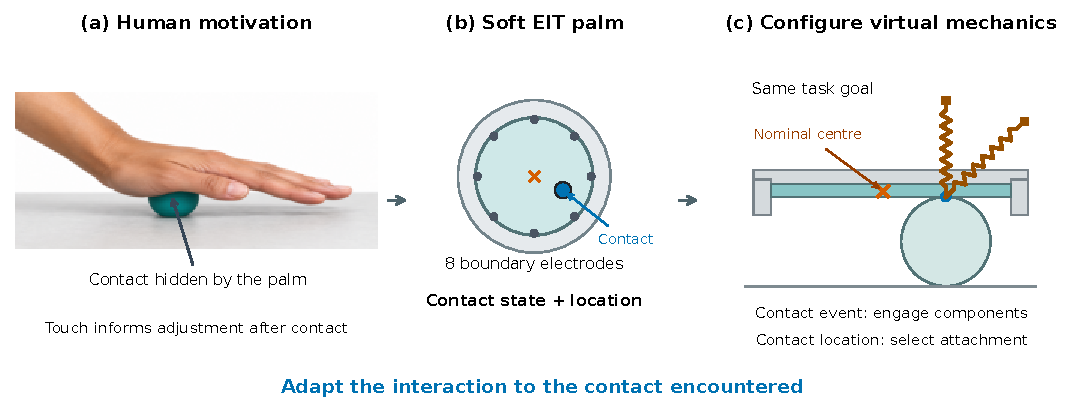
\includegraphics[width=0.98\textwidth]{figures/framework.pdf}
\caption{Tactile configuration of virtual mechanics. (a) Occluded palm contact motivates sensing; this AI-generated illustration is not an experiment. (b) The proposed EIT palm supplies contact state and location. (c) Contact selects engagement and the virtual attachment. For the joystick, EIT defines the VMC attachment at contact; for the ball, the attachment can update during rolling. Springs represent software components.}
\label{fig:framework}
\end{figure*}

\section{Related Work}
EIT infers contact information from boundary electrical measurements~\cite{zhang}. Economy of Touch connects measurement budgets to tactile inference tasks~\cite{xu}; here we examine the consequences of imperfect estimates in a specified controller. Tactile manipulation already includes predictive control of balls and analogue sticks~\cite{tian}, and compliant rolling with contact and wrench feedback~\cite{weng}. Application choice alone therefore does not establish novelty.

VMC expresses control through virtual components~\cite{pratt}; dynamic virtual mechanisms and their passivity-based design are developed in~\cite{larby}, with recent application to uncertain reaching~\cite{reaching}. Moving compliant interaction to sensed contact also has direct precedents: Kang et al. relocate a compliance centre using force/torque-based localization~\cite{kang}; Kappassov et al. combine tactile features with Cartesian impedance~\cite{kappassov}; Kleff et al. formulate control at the centre of pressure~\cite{kleff}. Recent preprints estimate interaction frames from ultrasound~\cite{arefin} and optical tactile sensing~\cite{rapuano}.

Our spatial intervention changes the attachment origin and Jacobian while holding gains fixed. A spring--damper at that contact can be equivalent to contact-frame impedance. The virtual carriage additionally receives coupling reaction and has internal dynamics, which an equivalent dynamic impedance controller could reproduce. We therefore test the contribution of EIT information to attachment and virtual-state correction, without attributing superiority to controller representation.

\section{Tactile Configuration of Virtual Mechanics}
\subsection{Contact geometry and force allocation}
The proposed palm has a 90 mm active disk, eight electrodes, and a recessed housing of diameter 130 mm and thickness 33.5 mm. The interface returns contact validity, timestamp, and one compact contact location $\hat c=(\hat x,\hat y,z_s)$ in the palm frame. The nominal face coordinate $z_s$ is calibrated. Multiple contacts require an extended estimator.

For joint coordinates $q$ and palm pose $(p_E,R_E)$, the selected attachment and material-point Jacobian are
\begin{equation}
 p_c=p_E+R_E\hat c,\qquad
 J_c=J_v-\crossmat{R_E\hat c}J_\omega.
\end{equation}
The material velocity $J_c\dot q$ excludes apparent motion from contact migration. A spring--damper couples this point to a task reference $h(z)$:
\begin{equation}
 f_c=P_t\{K_c[h(z)-p_c]+D_c[G\dot z-J_c\dot q]\},
 \quad G=\partial h/\partial z.
 \label{eq:coupling}
\end{equation}
Here $P_t$ selects horizontal directions, with stiffness 700 N/m, damping 30 Ns/m, and component force limited to $\pm3$ N. A separate normal spring--damper supplies nominal 3 N preload. With total force $f_v$, the ideal torque-controlled model applies
\begin{equation}
 \tau=J_c^T f_v+J_\omega^T(K_R e_R-D_R\omega)
       +h_b(q,\dot q)-B_q\dot q,
\end{equation}
where $h_b$ compensates model bias and $B_q$ adds joint damping. Orientation control and torque limits are shared within comparisons. This model does not establish direct torque-control availability on physical UR3e hardware.

An attachment error changes the force moment by $(R_E(\hat c-c))\times f_v$. For a planar body under imposed load $F$, linear stiffness $K_y$ and rotational stiffness $K_\phi$ give
\begin{equation}
 y_c=F/K_y+F(\hat r-r)^2/K_\phi,
 \label{eq:bias}
\end{equation}
where $r$ and $\hat r$ are actual and selected offsets. Attachment mismatch adds displacement through rotation. Strong orientation control can suppress this effect; the model predicts a conditional benefit under finite rotational compliance. The companion simulation report documents separate loading and supported-reorientation checks; the task comparisons below provide the main evidence.

\subsection{Engagement and attachment updates}
A bounded approach reference precedes engagement, preload and interaction. At 20 Hz, three consecutive electrical frames above threshold trigger engagement; two below a lower threshold trigger loss. Electrical triggers are not vetoed by true contact. Premature engagement counts as failure. The recovery policy brakes, lifts, repositions and reacquires contact.

For the joystick, EIT defines the VMC attachment at contact, and the attachment remains fixed in the palm frame during manipulation. Ball attachment updates are filtered and bounded. Changing $\hat c^-$ to $\hat c^+$ rebases the anchor as
\begin{equation}
 a^+=a^-+R_E(\hat c^+-\hat c^-),
\end{equation}
preserving spring extension at the update. This avoids an instantaneous force jump from changing coordinates, but does not prove passivity of the sampled controller.

\subsection{Joystick and ball task structures}
Figure~\ref{fig:vmctasks} shows the virtual structures and simulated setups. The commanded joystick angle $\theta_d$ sets both the prescribed arc reference $h(\theta_d)$ and the desired palm orientation; $\theta$ denotes the actual joystick angle. The arc is initialized at the selected attachment and follows $+12$ then $-12$ degrees. In the general coupling equation, $z=\theta_d$. Both conditions receive the same axis and effective radius of 92 mm (80 mm pivot-to-cap-centre length plus 12 mm cap radius). Palm orientation control uses rotational stiffness 3 Nm/rad and damping 1 Nms/rad. EIT supplies contact location; it neither identifies the pivot or length nor measures joystick angle. This controller includes moving-reference, orientation and preload components.

For the ball, virtual carriage coordinate $z=s$ represents estimated centre progress along unit direction $t$. Its output $h(s)=h_0+2t(s-s_0)$ gives $G=2t$ and dynamics
\begin{equation}
 M_v\ddot z=u_g(z_g-z)-d_v\dot z-G^T f_c.
 \label{eq:virtualstate}
\end{equation}
Virtual mass is 0.6 kg, damping 6 Ns/m and speed limit 12.5 mm/s. The bounded goal effort drives motion, while coupling reaction can slow it. The factor two approximates rolling between a stationary table and translating palm. Actual sphere rotation and slip follow physical contact dynamics without an enforced rolling constraint.

At each valid frame, $\bar x_b^+=0.65\bar x_b^-+0.35(p_E+R_E\hat c)_x$ filters the estimated ball position. The state correction is $\delta z=\operatorname{clip}[0.20(\bar x_b-z),\pm3\,\mathrm{mm}]$, with $z^+=z^-+\delta z$ and $h_0^+=h_0^--2t\delta z$. Thus task progress changes while coupling extension is preserved. Estimating the ball centre from contact assumes a near-horizontal palm. The position-feedback comparison substitutes another observation while retaining this correction rule.

\begin{figure*}[t]
\centering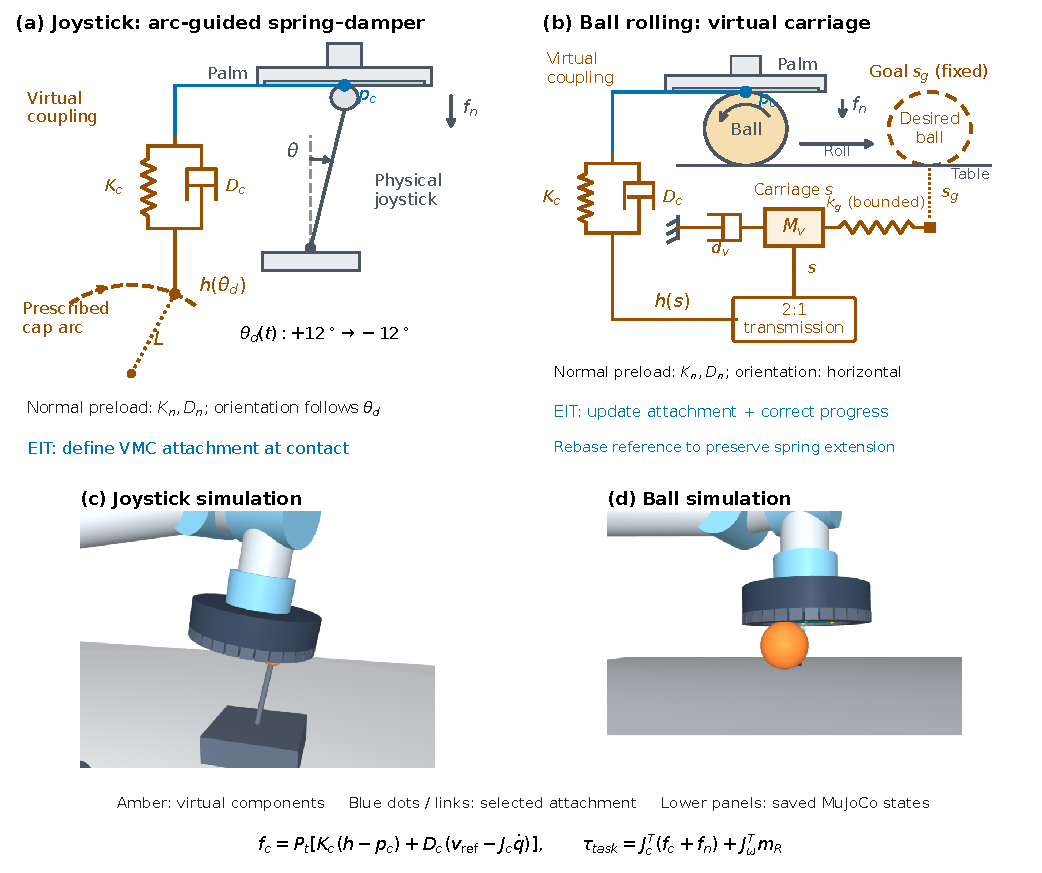
\includegraphics[width=0.98\textwidth]{figures/task_setup_mechanisms.pdf}
\caption{Task structures with the palm above the object. (a) Joystick: a spring--damper couples the selected attachment to a prescribed arc; EIT defines the VMC attachment at contact. The angle $\theta$ is measured from the dashed upright reference to the shaft about its pivot. (b) Ball: the dashed ball marks the fixed desired centre position $s_g$. Its goal spring drives carriage $s$ with mass and damping; a 2:1 transmission connects the carriage to reference $h(s)$, with solid links representing bidirectional mechanical coupling. The dotted guide links the goal position to its spring reference. Both tasks include normal preload and orientation control; $v_{\mathrm{ref}}$ is the commanded reference velocity. (c,d) Saved MuJoCo states for the corresponding controllers. Geometry and contact properties are assumed.}
\label{fig:tasksetups}\label{fig:vmctasks}
\end{figure*}

\section{Shared Simulation and Sensing Setup}\label{sec:setup}
\subsection{Robot, objects and evaluation}
The six-joint UR3e model uses official link transforms and inertial parameters~\cite{ur} in MuJoCo~\cite{mujoco}, with 1 ms dynamics, ideal torque actuation and exact bias compensation. Unilateral frictional contact permits slip and separation. Device mass is 0.35 kg. The assumed joystick has $\pm20$ degree travel and 0.15 Nm/rad return stiffness. The ball has diameter 50 mm and mass 72 g, on a horizontal table with nominal friction coefficient 0.7. A segmented housing has an opening radius of 47 mm and a lip 3 mm beyond the pad. These mechanics and clearances require physical measurement.

The original campaign contains 540 trials; 27 additional centre-attachment joystick trials complete the matched prescribed-arc comparison with unchanged seeds, gains and criteria. Controller selection for the main presentation is retrospective. After 68 exploratory trials, the ball follow-up freezes 329 evaluation trials with disjoint sensor seeds and unchanged controller gains. All attempts enter completion counts. Independent simulated object and contact signals score performance and drive common protective guards; they do not supply task feedback. Ball conditions share initial camera initialization, with no vision during contact; recovery can obtain a between-stroke camera update.

\subsection{Synthetic EIT and learned decoder}
A two-dimensional finite-element model represents a conductive sheet of radius 45 mm with complete-electrode boundary conditions. Eight adjacent current drives and five non-drive voltage differences per drive give 40 channels, including reciprocal redundancy. A saturating conductance perturbation represents contact. The constitutive law, noise, hysteresis and 80 ms load response are assumptions; sampling is 20 Hz. This is a synthetic sensing model rather than a calibrated physical sensor.

A 100-tree Extra Trees decoder is trained on 480 synthetic contact episodes and selected using 80 validation episodes. Each episode has a new location within radius 37 mm and loads of 1, 3, 6, 3 and 1 N. Complete episodes and material sessions remain separate across splits. On 100 held-out episodes using a different mesh, median location error is 0.91 mm and the 95th percentile is 4.35 mm. Force mean absolute error is 0.94 N, rising to 1.45 N under material shift. Only location and electrical contact events enter control; training includes force labels, so this does not establish that force labels are unnecessary.

\section{Manipulation Results}\label{sec:tasks}
\subsection{Joystick: attachment accuracy and contact load}
\textit{Purpose and procedure.} Test operation from an off-centre landing without recentering the palm. Approach at 8 mm/s, detect contact, ramp preload, then command $+12$ and $-12$ degrees. Cross lateral offsets $-25,0,+25$ mm, initial pad-to-object clearances of 2, 6 and 14 mm, and three sensor seeds: 27 trials per attachment. The controller and contact detector are shared; only attachment selection changes.

Success requires both holds, mean joystick-angle error at most 2 degrees in the scoring windows, contact for at least 95\% of those windows, peak pad force at most 12 N, peak rim force below 0.2 N, and no premature engagement or protective stop. Shared guards stop above 15 N pad force, 1 N rim force or 5 rad/s joint speed.

EIT completes 27/27 trials; centre attachment completes 9/27, all at zero offset (Fig.~\ref{fig:taskresults}(a)). Eleven centre trials stop on rim contact and seven reach the time limit. Mean peak pad force is 4.19 N with EIT versus 5.61 N at the centre. Mean joystick-angle error is 0.32 degrees for EIT and 2.84 degrees for centre, but the latter is available for only 18/27 trials: nine stop before any scoring window. Thus the force and error differences are not comparisons at matched completion. The result depends on the specified orientation gains and recessed housing.

The prescribed arc was selected because the alternative reaction-driven virtual lever had larger mean angle error (1.29 versus 0.32 degrees), despite 27/27 completion for both. At return stiffness 0.05 Nm/rad, the lever completed 0/9 versus 9/9 for the prescribed arc. Extra virtual dynamics therefore have no established joystick advantage.

\subsection{Ball: position correction after a push}\label{sec:ballfollowup}
\textit{Purpose and procedure.} Test whether contact sensing corrects ball motion that robot travel cannot predict. Command a 20 mm roll for 8 s after engagement, with centre attachment and shared contact detection. Compare robot-motion, EIT-position and true-contact estimates. The robot-motion estimate adds half the palm's horizontal travel to the initial camera position, assuming rolling without slip. An unobserved 4 N forward force acts on the ball for 0.35 s, starting 2 s after engagement. Two offsets (0 and $+10$ mm) and four seeds give eight trials per condition.

Final ball position error is absolute target distance along the rolling direction, averaged over the final second (7--8 s after engagement). It measures task accuracy. Success requires this error at most 5 mm, mean final speed at most 4 mm/s, cross-path error at most 5 mm, load limits and no premature engagement or protective stop. Early terminations have no final-error score; regrasp is disabled.

Mean error falls from 2.73 mm for the robot-motion estimate to 0.41 mm for EIT and 0.05 mm for true contact (Fig.~\ref{fig:taskresults}(b)). All complete 8/8; EIT improves all eight paired errors at the same mean peak load of 3.61 N. A prescribed-reference controller also benefits from EIT (2.23 to 0.46 mm, 8/8 each), so this effect belongs to sensing rather than uniquely to carriage dynamics. A stronger 6 N push terminates all 24 attempts across the three estimates.

\subsection{Ball: updating a moving contact attachment}
\textit{Purpose and procedure.} Test whether attachment updates reduce palm tilt as contact migrates. All conditions share EIT position feedback. Compare palm centre, initial EIT contact, updated EIT contact and updated true contact. Cross offsets $+10,+25$ mm, orientation stiffnesses 0.3, 1 and 3 Nm/rad, and four seeds: 96 trials under the same 20 mm protocol.

At 0.3 Nm/rad, mean maximum palm tilt is 2.98, 4.01, 1.92 and 1.92 degrees respectively; each condition completes 8/8 (Fig.~\ref{fig:taskresults}(c)). Updating improves alignment, but mean peak load is 3.22 N versus 3.24 N for initial contact and 2.89 N for centre attachment. At 3 Nm/rad, the initial-versus-updated tilt difference narrows to 1.01 versus 0.94 degrees. All 16 additional $-25$ mm edge trials terminate. These results show a benefit under finite orientation compliance, with a geometric limit and no demonstrated completion increase.

A nominal 25 mm roll in the earlier campaign showed no attachment benefit: centre and updated EIT both completed 27/27, with mean camera-target errors of 0.18 and 0.32 mm. Both already received EIT position feedback. Full nominal, support and exploratory dynamics experiments remain in the companion simulation reports.

\begin{figure*}[t]
\centering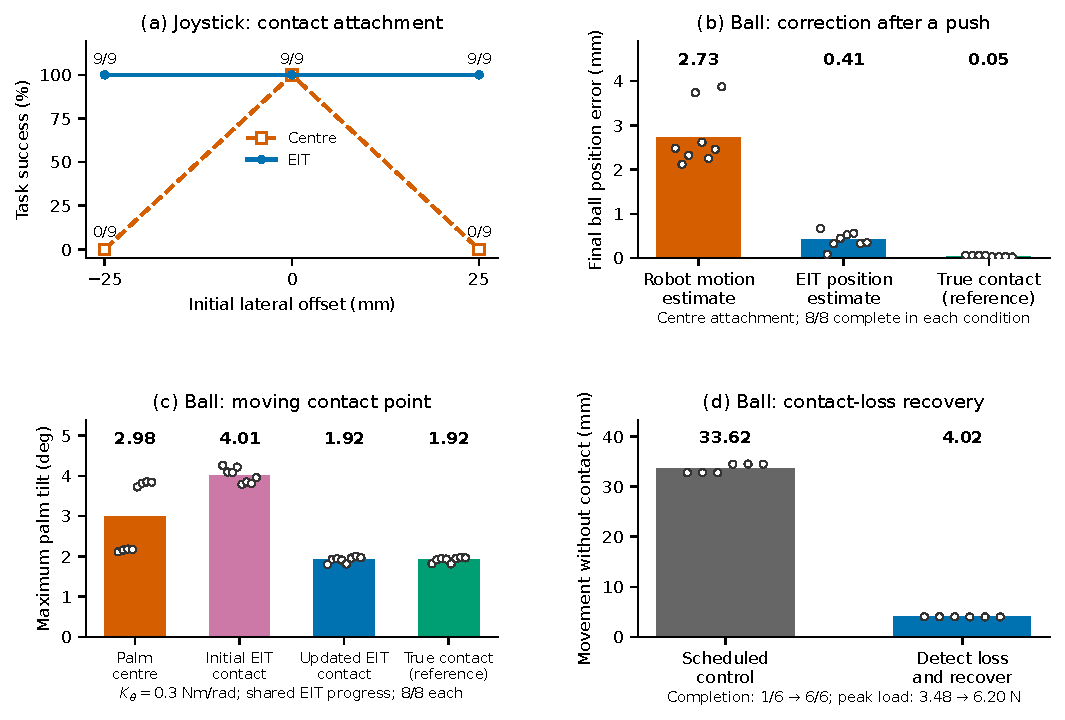
\includegraphics[width=0.98\textwidth]{figures/main_task_results.pdf}
\caption{Executed task comparisons. (a) Joystick completion: nine trials per offset. (b) Ball error after a push, averaged over the final second: eight trials per condition. Robot motion assumes ball travel is half the palm travel; true contact supplies a simulation reference. (c) Moving contact: initial EIT defines the VMC attachment at contact and keeps it fixed in the palm frame; updated EIT moves it during rolling, with shared EIT position feedback. Eight trials per condition at orientation stiffness 0.3 Nm/rad. (d) Contact-loss recovery: six trials per condition. Bars and numbers show means; white circles show individual trials. Marker shapes and direct labels supplement colour. All conditions in (b,c) complete. These synthetic trials do not establish hardware reliability.}
\label{fig:taskresults}\label{fig:ballfollowup}
\end{figure*}

\subsection{Ball: recovery after contact loss}
\textit{Purpose and procedure.} During a requested 60 mm roll, a fixture lowers the table by 20 mm over 0.15 s at 2.50 s, holds for 0.40 s and restores it over 1.20 s. The controller receives no fixture timestamp. Compare scheduled interaction with tactile detection followed by braking and reacquisition, using shared limits and six paired trials ($\pm10$ mm offsets, three seeds).

Tactile recovery completes 6/6 versus 1/6; mean palm movement without contact falls from 33.62 to 4.02 mm, while mean peak load rises from 3.48 to 6.20 N (Fig.~\ref{fig:taskresults}(d)). Mean detection response is 91 ms and sustained stopping occurs after about 405 ms. The electrical model returns immediately to baseline on detachment, so these times depend on that assumption. This comparison supports event handling and recovery; it does not isolate the value of changing virtual mechanism topology.

\section{Sensor Quality and Task Performance}\label{sec:quality}
\begin{figure}[t]
\centering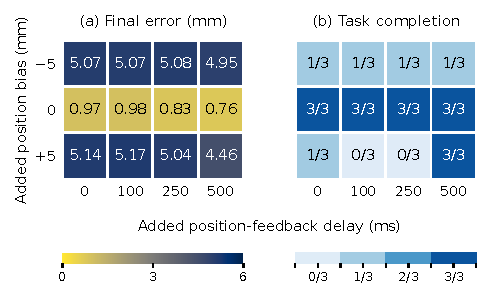
\includegraphics[width=\columnwidth]{figures/sensor_quality_results.pdf}
\caption{Synthetic position-feedback sensitivity during ball rolling after a push. Added bias and delay vary while centre attachment and contact detection remain shared. (a) Mean final position error over the final second. (b) Trials meeting all success criteria, including the 5 mm error limit; three seeds per cell.}
\label{fig:sensorquality}
\end{figure}
Figure~\ref{fig:sensorquality} summarizes 36 ball trials crossing position biases $-5,0,+5$ mm with added delays of 0, 100, 250 and 500 ms, using three seeds per cell. Positions are transformed with the pose at sampling before queuing; centre attachment and contact detection remain shared. With zero added bias, all three trials pass at every delay. At zero added delay, either sign of 5 mm bias leaves 1/3 passing and approximately 5.1 mm mean final position error. With $+5$ mm bias, completion varies from 0/3 at 100--250 ms to 3/3 at 500 ms, so delay effects are condition-dependent. Nine further trials suppress position updates for 0.5, 1 or 2 s during the push; all complete after updates resume, with contact events still available. High electrical noise in a separate six-trial test causes false engagement and failure in every trial.

Bias near the task tolerance is therefore consequential, while this slow task tolerates substantial position-feedback delay. The results do not establish a universal latency limit or recovery from complete sensing loss. In four representative trials, halving the physics step preserves completion and changes final error by at most 0.00493 mm. Saved trajectories and numerical checks accompany the reports.

For physical training, measure signed bias and error tails on curved and edge contacts, with complete sessions held out. Timestamp alignment and contact-event reliability should be assessed alongside localization. Overlay measured errors on task-performance tests before selecting a required sensing accuracy or rate; the present synthetic sweep does not establish physical operating specifications.

\section{Discussion and Validation Priorities}
The joystick results support EIT attachment within the tested controller and housing. Ball results distinguish position correction from attachment updates. Neither establishes a general advantage of VMC over impedance control. In exploratory stop--restart trials, the carriage reduced overshoot but increased integrated error; a matched-responsiveness advantage remains unproven.

Orientation compliance requires a task-level justification. Stronger orientation control can reject attachment-induced moments. The decisive next comparison is centre attachment versus EIT across orientation gains, measuring task accuracy and contact force together. Lower force at comparable completion would support a practical benefit. The present joystick force reduction accompanies different completion rates, and ball attachment updates do not reduce load relative to centre attachment. Geometry-error tests should hold the assumed joystick length and axis fixed while perturbing the physical object; current trials supply matching geometry.

Hardware validation requires curved-contact EIT calibration, measured bracket clearance and friction, and a verified robot interface. Prioritize the same joystick and ball comparisons with independent angle, ball-motion and force references, paired conditions across sessions and all attempts retained. Ideal actuation, assumed electrical/contact mechanics and synthetic seeds limit transfer. Attachment rebasing and state correction preserve instantaneous coupling extension, but sampled switching, clipping and adaptation still require analysis before a passivity guarantee.

\section{Conclusion}
EIT contact information configures virtual attachments and corrects task progress in simulated joystick and ball manipulation. It improves joystick completion, corrects ball-position error after a push and reduces palm tilt during contact migration at low orientation stiffness. Sensing-bias tests expose a task-dependent limitation. The evidence motivates physical calibration and matched accuracy--load comparisons while retaining known geometry and controller assumptions.

\begin{thebibliography}{99}
\bibitem{jenmalm} P. Jenmalm and R. S. Johansson, ``Visual and somatosensory information about object shape control manipulative fingertip forces,'' \emph{Journal of Neuroscience}, vol. 17, no. 11, pp. 4486--4499, 1997, doi: 10.1523/JNEUROSCI.17-11-04486.1997.
\bibitem{pratt} J. Pratt, C.-M. Chew, A. Torres, P. Dilworth, and G. Pratt, ``Virtual model control: An intuitive approach for bipedal locomotion,'' \emph{Int. J. Robotics Research}, vol. 20, no. 2, pp. 129--143, 2001, doi: 10.1177/02783640122067309.
\bibitem{larby} D. Larby and F. Forni, ``Optimal virtual model control for robotics: Design and tuning of passivity-based controllers,'' arXiv:2411.06627, version 3, 2025, preprint.
\bibitem{zhang} H. Zhang, A. Kalra, A. Lowe, Y. Yu, and G. Anand, ``A hydrogel-based electronic skin for touch detection using electrical impedance tomography,'' \emph{Sensors}, vol. 23, no. 3, art. 1571, 2023, doi: 10.3390/s23031571.
\bibitem{xu} X. Xu, D. Hardman, and F. Iida, ``Economy of Touch: Task-driven information selection in electrical impedance tomography-based tactile robotic sensing,'' \emph{Advanced Intelligent Systems}, vol. 8, no. 7, art. e202501493, 2026, doi: 10.1002/aisy.202501493.
\bibitem{tian} S. Tian, F. Ebert, D. Jayaraman, M. Mudigonda, C. Finn, R. Calandra, and S. Levine, ``Manipulation by feel: Touch-based control with deep predictive models,'' in \emph{Proc. IEEE ICRA}, 2019, doi: 10.1109/ICRA.2019.8794219.
\bibitem{weng} H. Weng, Y. Chen, and K. M. Lynch, ``Compliant in-hand rolling manipulation using tactile sensing,'' arXiv:2603.04301, 2026, preprint.
\bibitem{reaching} Y. Zhang, D. Larby, F. Iida, and F. Forni, ``Virtual model control for compliant reaching under uncertainties,'' arXiv:2610.05695, 2026, preprint.
\bibitem{kang} S. Kang, Y. K. Hwang, M. Kim, C. Lee, and K.-I. Lee, ``A compliant controller dynamically updating the compliance center by contact localization,'' \emph{Robotica}, vol. 16, no. 5, pp. 543--550, 1998, doi: 10.1017/S0263574798000058.
\bibitem{kappassov} Z. Kappassov, J. A. Corrales-Ramon, and V. Perdereau, ``Touch driven controller and tactile features for physical interactions,'' \emph{Robotics and Autonomous Systems}, vol. 123, art. 103332, 2020, doi: 10.1016/j.robot.2019.103332.
\bibitem{kleff} S. Kleff, L. Joseph, and V. Padois, ``Geometrically consistent tactile servoing via hybrid force--position control at the center of pressure,'' \emph{IEEE Robotics and Automation Letters}, 2026, doi: 10.1109/LRA.2026.3699162.
\bibitem{arefin} M. M. Arefin and M. E. Tiryaki, ``Contact-aware impedance controller for robot-assisted ultrasound imaging,'' arXiv:2609.34400, 2026, preprint.
\bibitem{rapuano} A. Rapuano, S. Orelli, B. Bazzana, A. Franchi, and A. De Luca, ``Tactile reconstruction of contact task frames and forces for hybrid force/motion control,'' arXiv:2610.10020, 2026, preprint.
\bibitem{ur} Universal Robots, \emph{Universal Robots ROS2 Description}, commit d4042c1f5123c86645cc5dbd650b4f461f697ee9, 2026. \url{https://github.com/UniversalRobots/Universal_Robots_ROS2_Description}.
\bibitem{mujoco} E. Todorov, T. Erez, and Y. Tassa, ``MuJoCo: A physics engine for model-based control,'' in \emph{Proc. IEEE/RSJ IROS}, 2012, pp. 5026--5033, doi: 10.1109/IROS.2012.6386109.
\end{thebibliography}
\end{document}
